\section{Auswertung}
\label{sec:Auswertung}
\subsection{Magnetische Flußdichte zweier Spulen}

\begin{table}[H]
  \centering
  %\caption{Messwerte x und y sowie das Ergebnis nach Gleichung blabla.}
  \csvreader[tabular=c|c,
  head=false, 
  table head= $I\:/\:\si{\centi\meter}$ & $B\:/\:\si{\milli\tesla}$ \\\midrule,
  late after line= \\]
  {LSpule.csv}{1=\eins, 2=\zwei}{$\num{\eins}$ & $\num{\zwei}$}
  \label{tab:messwerte}
\end{table}

Die Messwerte für die magnetische Flußdichte der 
langen Spule sind in Tabelle (REFERENZ) aufgelistet.
Außerdem sind sie zusammen mit dem Theoriewert, welcher
sich nach Gleichung(REFERENZ) als
\begin{equation}
  B_{L,t}=1,909\,\si{\milli\tesla}\nonumber
\end{equation}
berechnen lässt, in Abbildung(REFERENZ) in einem
xB-Diagramm aufgetragen, wobei der Nullpunkt
von x am Anfang der Spule liegt. 

\begin{table}[H]
  \centering
  %\caption{Messwerte x und y sowie das Ergebnis nach Gleichung blabla.}
  \csvreader[tabular=c|c,
  head=false, 
  table head= $I\:/\:\si{\centi\meter}$ & $B\:/\:\si{\milli\tesla}$ \\\midrule,
  late after line= \\]
  {KSpule.csv}{1=\eins, 2=\zwei}{$\num{\eins}$ & $\num{\zwei}$}
  \label{tab:messwerte}
\end{table}

\begin{figure}[H]
  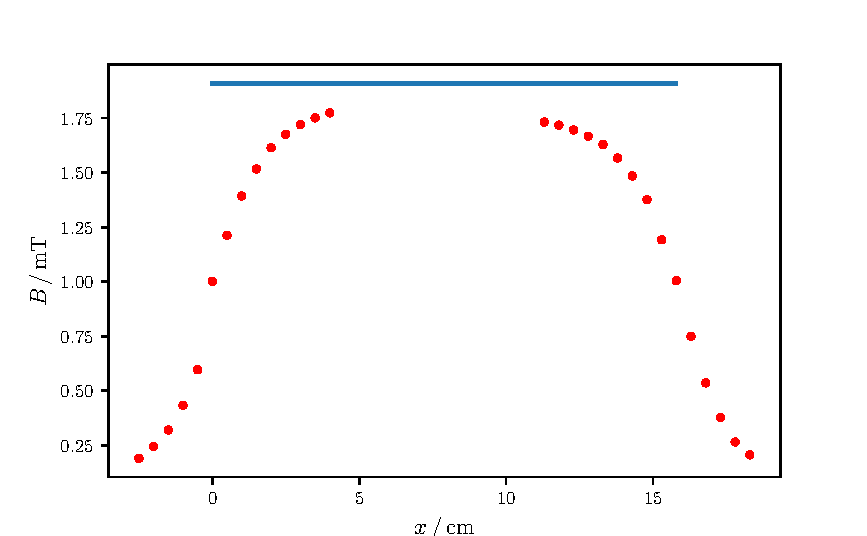
\includegraphics{plot1-1.pdf}
\end{figure}
\noindent Beim Vergleich mit der Theorie fällt auf, dass
die gemessenen Werte noch in der Spule am Randbereich
abfallen und auch in der Mitte nicht ganz den vollen
Theoriewert erreichen.




\subsection{Magnetische Flußdichte eines Helmholzspulenpaares}
\subsection{Hysteresekurve einer Spule mit Eisenkern}

\begin{table}[H]
  \centering
  %\caption{Messwerte x und y sowie das Ergebnis nach Gleichung blabla.}
  \csvreader[tabular=c|c|c,
  head=false, 
  table head= $I\:/\:\si{\ampere}$ & $B\:/\:\si{\milli\tesla}$ & $H \:/\: \si{\ampere}$ \\\midrule,
  late after line= \\]
  {tabelle1.csv}{1=\eins, 2=\zwei, 3=\drei}{$\num{\eins}$ & $\num{\zwei}$ & $\num{\drei}$}
  \label{tab:messwerte}
\end{table}

\begin{figure}
  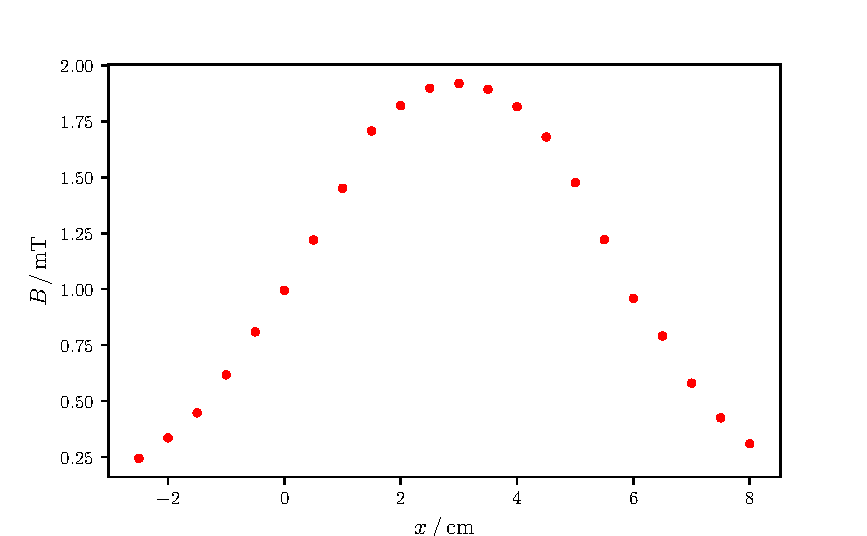
\includegraphics{plot1-2.pdf}
\end{figure}
\begin{figure}
  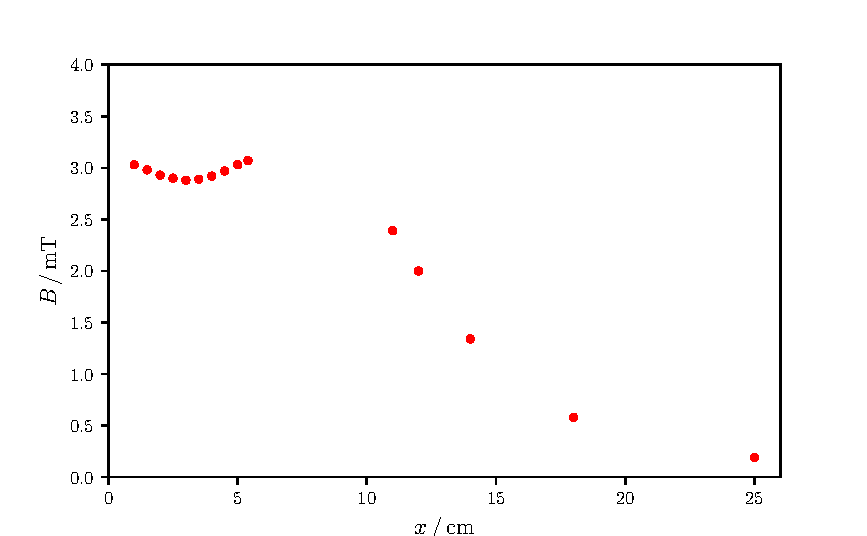
\includegraphics{plot2-1.pdf}
\end{figure}
\begin{figure}
  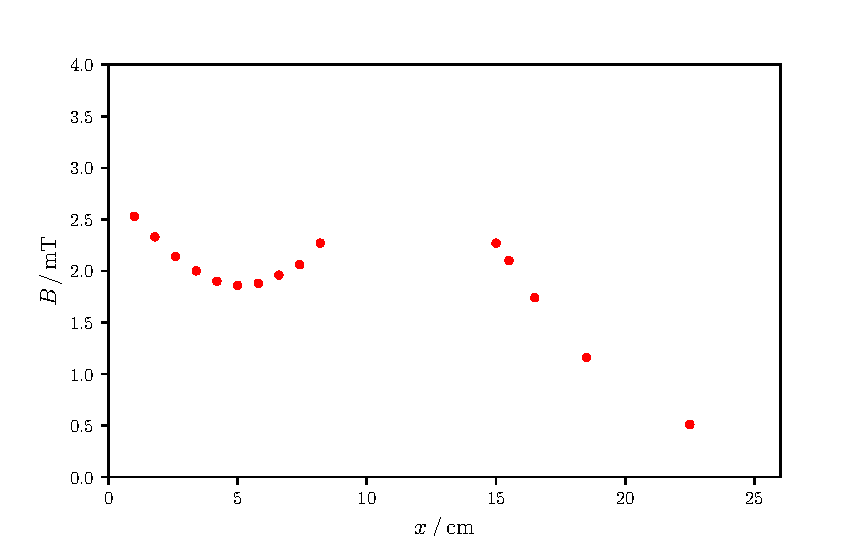
\includegraphics{plot2-2.pdf}
\end{figure}
\begin{figure}
  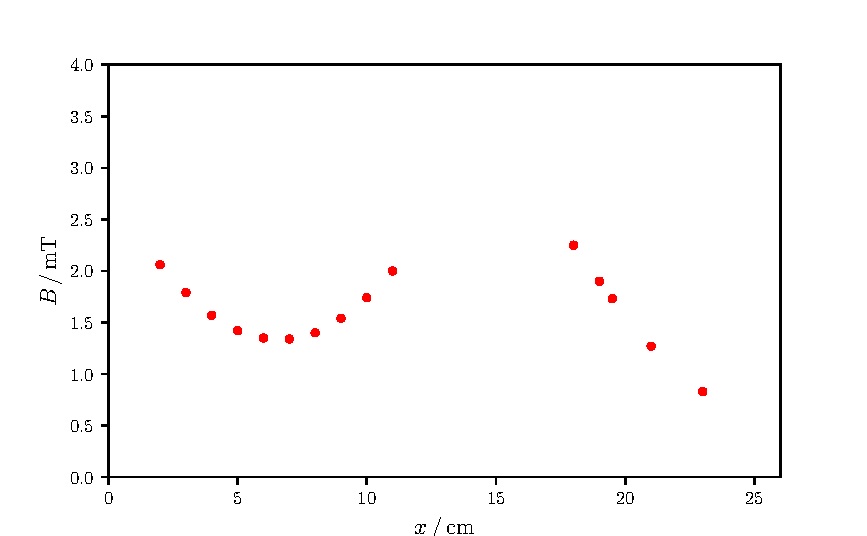
\includegraphics{plot2-3.pdf}
\end{figure}
\begin{figure}
  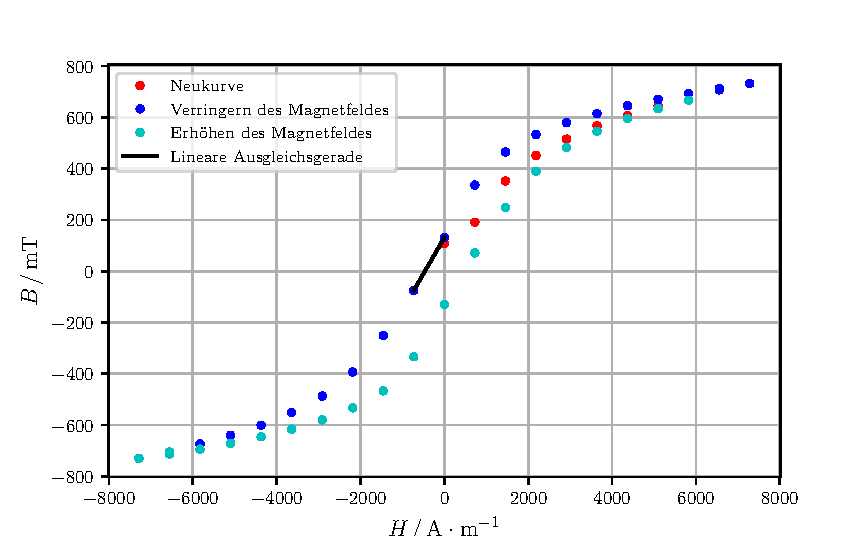
\includegraphics{plot3.pdf}
\end{figure}


